% Provenance (never printed): see sources/outline_sources.md (Year 2: viscosity, density and
% volatiles of magmas; magma ascent; dykes, sills and plutons; contact aureoles).
% Curves from figdata/bachelor-2/magma.py (GRD 2008 viscosity, DensityX density, Moore 1998
% solubility data, erf sill cooling, Stefan solidification); exercise and problem values in
% the Book 4 scratch calculators calc/ch05.py and calc/ch05pb.py.
\chapter{岩浆及其侵位}\label{ch:b2:magma-emplacement}

温度为 \qty{1200}{\celsius} 的玄武质熔体，流动时黏度约为
\qty{70}{Pa.s}，黏稠，但能够流淌。干燥的流纹质熔体在 \qty{800}{\celsius}
时黏度接近 \qty{e11}{Pa.s}，一块这样的熔体要数小时才会在自重下
明显下垂。两者相差十个数量级，甚至超过水与玄武岩之间的差距，
其差别主要来自两个因素：一是使熔体连成网络的二氧化硅，二是温度，
而硅质\omterm{def:b2:magma-emplacement:magma}{岩浆}的温度低数百度。百分之几的
溶解水（流纹质\omterm{def:b2:magma-emplacement:magma}{岩浆}在深部可以容纳）使其黏度降低为
原来的 \num{e5} 分之一；\omterm{def:b2:magma-emplacement:magma}{岩浆}上升时，水又以气泡形式析出，
黏度随之回升。这些数值决定\omterm{def:b2:magma-emplacement:magma}{岩浆}是平静地抵达地表，
还是爆发，抑或在地下数千米处凝固为\omterm{def:b2:magma-emplacement:bodies}{岩墙}、\omterm{def:b2:magma-emplacement:bodies}{岩床}或\omterm{def:b2:magma-emplacement:bodies}{深成岩体}。
本章把\omterm{def:b2:magma-emplacement:magma}{岩浆}当作一种材料，讨论其密度、黏度和挥发分，
\omterm{def:b2:magma-emplacement:magma}{岩浆}经裂隙上升及以团块形式上升的物理过程，
\omterm{def:b2:magma-emplacement:magma}{岩浆}停止时形成的形状，
以及它向周围岩石传递的热量。
% ledger: grd08:model, grd08:range, moore98:melts

\begin{recall}
\textbf{黏性流动}（物理系列本科二年级分册）：在黏度为 $\eta$ 的牛顿流体中，
切应力等于 $\eta$ 乘以速度梯度；两平行壁之间的压强梯度
驱动形成抛物线形（平面泊肃叶）剖面；慢速穿过黏性流体运动的球体
所受斯托克斯阻力为
$6\pi\eta a v$。\textbf{热传导}（同一分册）：温度满足
$\partial T/\partial t = \kappa\,\partial^2T/\partial x^2$，热扩散率 $\kappa = k/(\rho
c)$，温度阶跃按误差函数扩散，扩散距离的
量级为 $\sqrt{\kappa t}$。\textbf{浮力}（物理系列本科一年级分册）：浸没在
较密流体中的物体所受合力竖直向上，其大小等于被排开流体的
重量减去自身的重量。\textbf{化学平衡}（化学教材）：平衡时，
产物与反应物的活度满足质量作用定律，
其中常数 $K$ 随温度而变。来自本系列本科一年级分册的
静岩压力 $p = \rho g z$ 与地温线，
以及高中分册中的镁铁质岩与长英质岩、斑晶与斑状结构。
\end{recall}

\section{岩浆是什么}

\begin{definition}[岩浆]\label{def:b2:magma-emplacement:magma}
称\emph{岩浆}\index{岩浆}为地表以下熔融或部分熔融的岩石，即一种
\emph{硅酸盐熔体}\index{硅酸盐熔体}，即主要由硅、
氧和金属阳离子构成的液体，连同其所携带的任何晶体与气泡。
称\emph{晶粥}\index{晶粥}为晶体含量极高的岩浆，使晶体
彼此相接并构成骨架，不能像液体那样流动，其熔体只能
通过晶体之间的孔隙运移。
\end{definition}

熔体的成分与岩石一样，以
氧化物的质量百分数表示。本章始终以三种熔体为参照，它们
均经实验室研究：一种取自洋中脊的拉斑玄武岩
（约 \qty{51}{\percent} SiO$_2$，\qty{12}{\percent} 氧化铁，\qty{7}{\percent}
MgO），一种安山岩（\qty{63}{\percent} SiO$_2$），以及一种流纹岩（\qty{78}{\percent}
SiO$_2$，\qty{8}{\percent} Na$_2$O $+$ K$_2$O，几乎不含铁和镁）。
它们的喷发温度与成分一样差异显著：玄武质
\omterm{def:b2:magma-emplacement:magma}{岩浆}在 \qtyrange{1000}{1200}{\celsius} 喷出（在基拉韦厄火山流经熔岩管的熔岩
曾测得接近 \qty{1200}{\celsius}），安山质\omterm{def:b2:magma-emplacement:magma}{岩浆}在
\qtyrange{800}{1000}{\celsius}，流纹质\omterm{def:b2:magma-emplacement:magma}{岩浆}在 \qtyrange{650}{800}{\celsius} 喷出。
流纹质\omterm{def:b2:magma-emplacement:magma}{岩浆}温度较低，因为它是长期结晶作用的残余
或是地壳岩石的首次熔融产物，两者都发生在低温条件下
（见\cref{ch:b2:magmatic-differentiation}）。
% ledger: moore98:melts, tulane:magma-types, earle:kilauea-lava

晶体含量决定\omterm{def:b2:magma-emplacement:magma}{岩浆}能否流动。大型花岗岩体的野外与年代学研究
得出结论：整体\omterm{def:b2:magma-emplacement:magma}{岩浆}流动至少需要熔体分数
不低于 \qtyrange{30}{50}{\percent}（按体积计）；低于此值时，
晶体与相邻晶体胶结在一起，物质以固体形式变形，孔隙中充满熔体。
地壳中储存的\omterm{def:b2:magma-emplacement:magma}{岩浆}大部分被认为处于
这种状态，呈\omterm{def:b2:magma-emplacement:magma}{晶粥}形式，在热\omterm{def:b2:magma-emplacement:magma}{岩浆}自下方加入时
重新具有流动性。
% ledger: glazner04:tuolumne

\section{密度与黏度}

\subsection{熔体的密度}

\omterm{def:b2:magma-emplacement:magma}{硅酸盐熔体}没有晶格，但其体积仍可由各组分
的贡献求得。大量熔体的实验表明，每种氧化物都贡献
一个近似固定的每摩尔体积，即偏摩尔体积，其随温度与压强
的变化缓慢且线性；熔体的体积即这些贡献之和。
下表给出本章所用的数值。

\begin{table}[ht]
\centering\small
\begin{tabular}{lrrr}
\hline
氧化物 & $\bar V_i$ (\unit{cm^3/mol}) & $\partial\bar V_i/\partial T$ (\num{e-3}\,\unit{cm^3/(mol.K)}) & $\partial\bar V_i/\partial p$ (\num{e-4}\,\unit{cm^3/(mol.bar)}) \\
\hline
SiO$_2$  & 26.86 & 0     & $-1.89$ \\
Al$_2$O$_3$ & 37.42 & 2.62 & $-2.26$ \\
FeO      & 12.68 & 3.69  & $-0.45$ \\
MgO      & 12.02 & 3.27  & $0.27$ \\
CaO      & 16.90 & 3.74  & $0.34$ \\
Na$_2$O  & 29.65 & 7.68  & $-2.40$ \\
K$_2$O   & 47.28 & 12.08 & $-6.75$ \\
H$_2$O   & 22.9  & 9.5   & $-3.20$ \\
\hline
\end{tabular}
\caption{\omterm{def:b2:magma-emplacement:magma}{硅酸盐熔体}中氧化物组分的偏摩尔体积，
在 \qty{1}{bar} 下，连同其对温度和压强的导数。参考
温度 \qty{1773}{K}（FeO 为 \qty{1723}{K}，H$_2$O 为 \qty{1273}{K}）。数据：
DensityX 程序汇编（Iacovino and Till, 2019）。}
\label{tab:b2:magma-emplacement:volumes}
\end{table}
% ledger: densityx:volumes

\begin{proposition}[硅酸盐熔体的密度]\label{prop:b2:magma-emplacement:density}
设熔体含氧化物组分 $i$，其摩尔分数为 $X_i$，摩尔质量为
$M_i$ 与偏摩尔体积 $\bar V_i(T, p) = \bar V_i^{\circ} + (\partial\bar
V_i/\partial T)(T - T_{\mathrm{ref}}) + (\partial\bar V_i/\partial p)(p - p_{\mathrm{ref}})$.
若各组分在体积上理想混合，
\[
\rho = \frac{\sum_i X_i M_i}{\sum_i X_i \bar V_i(T,p)}.
\]
\end{proposition}

\begin{proof}
一摩尔熔体含 $X_i$ 摩尔组分 $i$，其质量为 $X_iM_i$。理想
体积混合意味着，每摩尔组分 $i$ 贡献体积 $\bar V_i$，与其他组分无关，
因此一摩尔熔体所占体积为 $\sum_i X_i\bar V_i$。
密度即二者之比。
\end{proof}

水的摩尔质量仅为 \qty{18}{g/mol}，而偏摩尔体积为
\qty{22.9}{cm^3/mol}，接近二氧化硅的值，它使熔体的密度
大幅降低。将本命题用于三种参考熔体，可得
玄武岩在 \qty{1200}{\celsius} 时为 \qty{2730}{kg/m^3}，安山岩在
\qty{1000}{\celsius} 时为 \qty{2480}{kg/m^3}，无水流纹岩在
\qty{850}{\celsius} 时为 \qty{2340}{kg/m^3}；溶解水含量为百分之一时，可使
玄武岩密度降低约 \qty{70}{kg/m^3}，相当于加热数百摄氏度的效果。
因此，玄武质熔体比其来源的地幔橄榄岩更轻
（参考地球模型中，地壳之下约为 \qty{3380}{kg/m^3}），并略轻于该模型的下地壳
（\qty{2900}{kg/m^3}），而流纹质熔体甚至
轻于其上地壳（\qty{2600}{kg/m^3}）。这一密度差驱动\omterm{def:b2:magma-emplacement:magma}{岩浆}
向上运动。
% ledger: densityx:volumes, densityx:water, data:prem

\subsection{黏度}

\omterm{def:b2:magma-emplacement:magma}{硅酸盐熔体}的黏度取决于 SiO$_4$ 四面体构成的网络，
四面体通过共享氧相连：熔体要流动，必须断开并重新形成
硅氧键。二氧化硅和氧化铝构成网络；镁、铁、钙和碱金属的
阳离子会破坏网络，水也是如此，它把桥氧转变为
羟基。对天然熔体的实验测量
结果跨越十五个以上数量级，从 \qty{0.1}{Pa.s} 到
\qty{e14}{Pa.s}，且它们并不遵循简单的阿伦尼乌斯定律，黏度
随 $1/T$ 增长的速度快于指数律，这发生在熔体冷却趋近其
玻璃化转变温度时。
% ledger: grd08:range

\begin{proposition}[福格尔–富尔彻–塔曼定律]\label{prop:b2:magma-emplacement:vft}
成分固定的\omterm{def:b2:magma-emplacement:magma}{硅酸盐熔体}，其黏度在十分之几个对数单位的精度内服从
下式：
\[
\log_{10}\eta = A + \frac{B}{T - C},
\]
其中 $\eta$ 以帕·秒计，$T$ 以开尔文计。对天然熔体，$A$ 接近
$-4.55$，与成分无关；$B$ 和 $C$（以开尔文计）为氧化物摩尔百分数的
线性组合，另含少数几个它们的乘积项，
由约 \num{1800} 个测量值拟合得到。
\end{proposition}
\admitted
% ledger: grd08:model, grd08:range

下图给出了该定律对三种参考熔体及含溶解水的
流纹岩的结果。在 \qty{1200}{\celsius} 时，玄武岩的
黏度 $\eta \approx \qty{70}{Pa.s}$；安山岩在 \qty{1000}{\celsius} 时约为
\qty{e6}{Pa.s}；无水流纹岩在 \qty{800}{\celsius} 时约为 $10^{10.9}$\,\unit{Pa.s}。
含水量为百分之四时，该流纹岩的黏度降至 $10^{5.5}$\,\unit{Pa.s}，
含水量为百分之六时降至 $10^{4.6}$\,\unit{Pa.s}。另一个仅由含水花岗质熔体
拟合的独立方程，所给数值与之相差在半个对数单位以内
（见\cref{exo:b2:magma-emplacement:1}）。水的影响在低温下最大，此时仅
零点几个百分点的含水量变化，就足以使黏度改变数个数量级。
% ledger: grd08:model, hd96:model, moore98:melts

\begin{omfigure}
\centering
\begin{tikzpicture}
\begin{axis}[omrecord, width=0.86\linewidth, height=6.4cm,
  xmin=600, xmax=1400, ymin=0, ymax=15,
  xlabel={温度 (\unit{\celsius})}, ylabel={$\log_{10}\eta$ (\unit{Pa.s})},
  legend pos=north east, legend style={font=\scriptsize},
  tick label style={font=\scriptsize}, label style={font=\small}]
\addplot[very thick, black, restrict x to domain=1000:1400] table[x=T_C, y=basalt] {figdata/out/bachelor-2-magma-visc.dat};
\addlegendentry{玄武岩，无水}
\addplot[very thick, brown, restrict x to domain=800:1300] table[x=T_C, y=andesite] {figdata/out/bachelor-2-magma-visc.dat};
\addlegendentry{安山岩，无水}
\addplot[very thick, red!70!black, restrict x to domain=650:1100] table[x=T_C, y=rhyolite] {figdata/out/bachelor-2-magma-visc.dat};
\addlegendentry{流纹岩，无水}
\addplot[thick, red!70!black, dashed, restrict x to domain=650:1000] table[x=T_C, y=rhy2] {figdata/out/bachelor-2-magma-visc.dat};
\addlegendentry{流纹岩，2 \% H$_2$O}
\addplot[thick, red!70!black, densely dotted, restrict x to domain=650:1000] table[x=T_C, y=rhy4] {figdata/out/bachelor-2-magma-visc.dat};
\addlegendentry{流纹岩，4 \% H$_2$O}
\addplot[thick, red!70!black, dashdotted, restrict x to domain=650:1000] table[x=T_C, y=rhy6] {figdata/out/bachelor-2-magma-visc.dat};
\addlegendentry{流纹岩，6 \% H$_2$O}
\end{axis}
\end{tikzpicture}
\par\smallskip{\small \omterm{def:b2:magma-emplacement:magma}{硅酸盐熔体}黏度随温度的变化，取自
福格尔–富尔彻–塔曼定律，其参数随成分而变，参数据
乔尔达诺、罗素和丁格韦尔（2008）。玄武岩：洋中脊拉斑玄武岩；
安山岩和流纹岩：实验室参考熔体（摩尔等人，1998）。每条
曲线只绘在该类\omterm{def:b2:magma-emplacement:magma}{岩浆}可保持熔融的温度范围内。}
\end{omfigure}
% ledger: grd08:model, moore98:melts

晶体会使\omterm{def:b2:magma-emplacement:magma}{岩浆}变得更加黏稠。刚性颗粒的悬浮体抵抗
剪切的能力比纯液体更强，因为液体必须绕过颗粒流动，
当颗粒密集到足以相互接触时，它们便锁定成
骨架结构。

\begin{proposition}[爱因斯坦–罗斯科关系]\label{prop:b2:magma-emplacement:roscoe}
由体积分数为 $\phi$ 的刚性球体组成的悬浮体，悬浮于
黏度为 $\eta_{\ell}$ 的牛顿流体中，其黏度为
\[
\eta = \eta_{\ell}\,(1 - R\phi)^{-2.5}, \qquad R = 1/\phi_m \approx 1.35,
\]
其中 $\phi_m$ 为最大堆积率，悬浮体在此时发生锁定。当
$\phi$ 较小时，此式化为爱因斯坦公式 $\eta = \eta_{\ell}(1 + 2.5\phi)$。
\end{proposition}
\admitted
% ledger: kolz22:einstein-roscoe

晶体含量为百分之二十时黏度加倍，百分之四十时黏度增至
七倍，百分之六十时增至六十倍以上（见\cref{exo:b2:magma-emplacement:5}）。在实际\omterm{def:b2:magma-emplacement:magma}{岩浆}中，晶体呈细长状且粒径多样，
锁定来得更早，约在 \qtyrange{50}{70}{\percent} 的晶体含量处，
即野外证据所确定的
整体流动终止点。

\section{挥发分}

\begin{definition}[岩浆挥发分]\label{def:b2:magma-emplacement:volatiles}
称\emph{岩浆挥发分}\index{岩浆挥发分}为\omterm{def:b2:magma-emplacement:magma}{岩浆}中的一种组分，
在深部溶于熔体，在低压下形成独立的气相：
主要是水，其次为二氧化碳，再次为硫的化合物。\emph{挥发分
出溶}\index{挥发分出溶}是指挥发分从
熔体中分出形成气泡。熔体的\emph{挥发分饱和
压力}\index{挥发分饱和压力}是指这样的压力：在其之下，
熔体中溶解的挥发分超过了其溶解度，因而必然形成气相。
\end{definition}

镁铁质\omterm{def:b2:magma-emplacement:magma}{岩浆}通常按质量计含 \qtyrange{1}{3}{\percent} 的挥发分，
中性\omterm{def:b2:magma-emplacement:magma}{岩浆}含 \qtyrange{3}{4}{\percent}，长英质\omterm{def:b2:magma-emplacement:magma}{岩浆}含
\qtyrange{4}{7}{\percent}，而出溶 \qtyrange{4}{6}{\percent} 的
水驱动了大多数爆炸式喷发。熔体能容纳多少水，首先取决于
压力。下图给出玄武质和
流纹质熔体的测量结果，这些熔体在已知水压下保持至饱和，随后淬火成
玻璃并加以分析：溶解度在低压下快速升高，
在高压下增长较慢。
% ledger: earle:volatiles, moore98:arc-water, moore98:h2o

\begin{proposition}[水的平方根定律]\label{prop:b2:magma-emplacement:sqrt}
设水在\omterm{def:b2:magma-emplacement:magma}{硅酸盐熔体}中主要以羟基形式溶解，
通过反应 $\mathrm{H_2O\,(gas)} + \mathrm{O^{2-}\,(melt)} \rightleftharpoons
2\,\mathrm{OH^-\,(melt)}$，熔体中的氧大量过量。则在
低水含量时，溶解水量与水压的平方根成正比，即
$w \approx s\sqrt{p}$，
其中 $s$ 为与熔体及温度有关的常数。
\end{proposition}

\begin{proof}
由质量作用定律得 $x_{\mathrm{OH}}^2 = K\,x_{\mathrm{O}}\,f$，其中 $f$ 为
水的逸度（在中等压力下接近其压强），$x$ 为
摩尔分数。熔体中的氧大量过量，因此
$x_{\mathrm{O}}$ 近似保持不变，于是 $x_{\mathrm{OH}} = \sqrt{Kx_{\mathrm{O}}}\,
\sqrt f$。每个溶解的水分子生成两个羟基，故溶解水量
为 $x_{\mathrm{OH}}/2$，与 $\sqrt f$ 成正比。含水量较高时，部分
水以分子形式溶解，其量与 $f$ 本身成正比，因而
溶解度增长快于平方根（见\cref{exo:b2:magma-emplacement:10}）。
\end{proof}

对测量数据作最小二乘拟合，$w = s\sqrt p$ 给出
玄武岩为 $s = 0.34$（重量百分比每 $\sqrt{\unit{MPa}}$），
流纹岩为 $s = 0.44$；每个测量值的含水量与其曲线的差值均在 1 个百分点以内。
含水 $w$ 重量百分比的熔体，其饱和压力为
$p_s = (w/s)^2$：含水 \qty{5}{\percent} 的流纹岩为 \qty{129}{MPa}，
相当于地壳中约 \qty{5}{km} 深处；含水 \qty{0.5}{\percent} 的玄武岩则只有
\qty{2}{MPa}，约相当于一百米或更浅。
% ledger: moore98:h2o

\begin{omfigure}
\centering
\begin{tikzpicture}
\begin{axis}[omrecord, width=0.8\linewidth, height=6cm,
  xmin=0, xmax=300, ymin=0, ymax=9,
  xlabel={水压 (\unit{MPa})}, ylabel={溶解 H$_2$O（重量分数，\%）},
  legend pos=south east, legend style={font=\scriptsize},
  tick label style={font=\scriptsize}, label style={font=\small}]
\addplot[very thick, red!70!black] table[x=P_MPa, y=rhyolite] {figdata/out/bachelor-2-magma-solub-fit.dat};
\addlegendentry{流纹岩，$0.44\sqrt p$}
\addplot[only marks, mark=*, mark size=2pt, red!70!black] table[x=P_MPa, y=w] {figdata/out/bachelor-2-magma-solub-rhyolite-data.dat};
\addlegendentry{流纹岩，实测}
\addplot[very thick, black] table[x=P_MPa, y=basalt] {figdata/out/bachelor-2-magma-solub-fit.dat};
\addlegendentry{玄武岩，$0.34\sqrt p$}
\addplot[only marks, mark=square*, mark size=2pt, black] table[x=P_MPa, y=w] {figdata/out/bachelor-2-magma-solub-basalt-data.dat};
\addlegendentry{玄武岩，实测}
\end{axis}
\end{tikzpicture}
\par\smallskip{\small 玄武质和流纹质熔体中水的溶解度，温度为
\qtyrange{800}{1200}{\celsius}，随水压的变化：实测数据
由摩尔等人（1998）汇编，并给出最小二乘平方根定律。在
\qty{100}{MPa}，约相当于地壳中 \qty{4}{km} 深处，流纹质熔体可含
\qty{4.4}{\percent} 的水，玄武质熔体可含 \qty{3.4}{\percent}。}
\end{omfigure}
% ledger: moore98:h2o

二氧化碳的溶解度远低于水。它在流纹质熔体中以分子形式溶解，
在玄武质熔体中以碳酸根形式溶解，在碱性熔体中的溶解量多于
拉斑玄武岩熔体，其溶解度同样随压力升高。同时含有两种气体的\omterm{def:b2:magma-emplacement:magma}{岩浆}
因此在深部便开始出溶，所出溶的气体富含 CO$_2$，
随着\omterm{def:b2:magma-emplacement:magma}{岩浆}上升，气体中水的比例逐渐升高。在深海底喷出的玄武岩
含有的气泡中 CO$_2$ 超过 \qty{95}{\percent}，这需要即使在
\qty{5}{km} 水深下仍达到 CO$_2$ 饱和。基拉韦厄火山亲本玄武岩的初始
CO$_2$ 含量估计在 \qtyrange{0.2}{0.6}{\percent} 之间，
而包裹在橄榄石晶体中的熔体包裹体
记录的饱和压力可达 \qty{500}{MPa}。
% ledger: lowenstern01:co2, lowenstern01:basalts

出溶气体占据很大的体积。在 \qty{900}{\celsius} 的\omterm{def:b2:magma-emplacement:magma}{岩浆}中，\qty{1}{\percent} 的水
若视为理想气体，其所占体积约为 \qty{100}{MPa} 下体积的 \qty{12}{\percent}，
在 \qty{10}{MPa} 时约为 \qty{57}{\percent}，在大气压强下超过
\qty{99}{\percent}（见\cref{exo:b2:magma-emplacement:7}）。气泡进一步降低
\omterm{def:b2:magma-emplacement:magma}{岩浆}密度，并使其上升更快；在黏性\omterm{def:b2:magma-emplacement:magma}{岩浆}中，气泡无法逸出，
这一点在\cref{ch:b2:eruptive-styles}中说明了气泡如何使\omterm{def:b2:magma-emplacement:magma}{岩浆}碎裂。

\section{上升}

密度小于外界的\omterm{def:b2:magma-emplacement:magma}{岩浆}体，所受的浮力为每单位体积
$\Delta\rho\,g$，其中 $\Delta\rho$ 为密度差。它
可以通过两种方式上升：一是沿其前方张开的裂隙，
二是以炙热而柔软的团块形式把周围岩石推开。

\subsection{岩墙}

在深部，岩石承受很大的静岩压力，但充满\omterm{def:b2:magma-emplacement:magma}{岩浆}的裂隙
压强略高于最小主应力时，便能
在其尖端张开并延伸。随着裂隙生长，\omterm{def:b2:magma-emplacement:magma}{岩浆}充填其中，结果
形成一片薄的\omterm{def:b2:magma-emplacement:magma}{岩浆}层，宽度为米级、长度为千米级，它
向上穿切岩石：这便是正在形成的\omterm{def:b2:magma-emplacement:bodies}{岩墙}。\omterm{def:b2:magma-emplacement:magma}{岩浆}随后在两近乎平行的
壁面之间流动。

\begin{proposition}[岩墙中岩浆的流动]\label{prop:b2:magma-emplacement:poiseuille}
黏度为 $\eta$ 的牛顿流体\omterm{def:b2:magma-emplacement:magma}{岩浆}，受压强梯度 $G$ 驱动向上运动，
（对于浮力流动，$G = \Delta\rho\,g$），在相距 $w$
的两平行壁面之间流动，其平均速度为
\[
\bar u = \frac{G w^2}{12\,\eta},
\]
\omterm{def:b2:magma-emplacement:bodies}{岩墙}单位长度的体积通量为 $q = \bar u w = G w^3/(12\eta)$。
\end{proposition}

\begin{proof}
在定常层流中，\omterm{def:b2:magma-emplacement:bodies}{岩墙}内的速度剖面为平面
泊肃叶抛物线 $u(x) = \frac{G}{2\eta}\left(\frac{w^2}{4} - x^2\right)$，适用于
$-w/2 \le x \le w/2$ 的范围，且在两壁面上为零。其平均值为
$\bar u = \frac1w\int_{-w/2}^{w/2}u\,dx = \frac{G}{2\eta}\left(\frac{w^2}{4} -
\frac{w^2}{12}\right) = \frac{Gw^2}{12\eta}$.
\end{proof}

\omterm{def:b2:magma-emplacement:bodies}{岩墙}宽度的三次方使宽\omterm{def:b2:magma-emplacement:bodies}{岩墙}远比窄\omterm{def:b2:magma-emplacement:bodies}{岩墙}高效。以下
例中，宽 \qty{1}{m} 的\omterm{def:b2:magma-emplacement:bodies}{岩墙}内，黏度为 \qty{100}{Pa.s} 的玄武岩，取 $\Delta\rho =
\qty{300}{kg/m^3}$，以约 \qty{2.5}{m/s} 的速度上升，一小时内即可穿过 \qty{10}{km} 的
地壳；同一\omterm{def:b2:magma-emplacement:bodies}{岩墙}中，黏度为 \qty{e6}{Pa.s} 的流纹岩则需要
一年以上，且会在途中凝固，因此硅质\omterm{def:b2:magma-emplacement:magma}{岩浆}需要宽得多的
\omterm{def:b2:magma-emplacement:bodies}{岩墙}（见\cref{exo:b2:magma-emplacement:6}）。这些流动的雷诺数 $\rho\bar u w/\eta$
很小，足以使其保持层流。喷发期间\omterm{def:b2:magma-emplacement:magma}{岩浆}上升速率的估计值，
可将低于约 \qty{0.1}{m/s} 的溢流式喷发与高于此值的
爆炸式喷发区分开来，两者之间存在过渡区间 \qtyrange{0.005}{0.25}{m/s}，
两种方式均可出现。金伯利岩来自深度超过
\qty{150}{km} 的深处，其上升速率估计为 \qtyrange{0.1}{30}{m/s}，
其中一例的扩散研究给出平均速率为 \qtyrange{0.02}{0.23}{m/s}，统计对象为
最后 \qtyrange{80}{110}{km} 的路程，历时 \numrange{5}{74} 天。
% ledger: cassidy18:ascent, casetta23:kimberlite

\subsection{底辟}

\begin{definition}[底辟、中性浮力面、岩浆顶蚀]\label{def:b2:magma-emplacement:ascent}
称\emph{底辟}\index{底辟}为一团浮力物质，即\omterm{def:b2:magma-emplacement:magma}{岩浆}或部分熔融的
岩石，借推开周围物质而上升。\omterm{def:b2:magma-emplacement:magma}{岩浆}的
\emph{中性浮力面}\index{中性浮力面}是其密度与周围岩石密度相等的
深度：其下方\omterm{def:b2:magma-emplacement:magma}{岩浆}具有浮力，
其上方则比周围岩石更致密。\emph{岩浆
顶蚀}\index{岩浆顶蚀}是指围岩或顶板岩块脱落，并沉入
\omterm{def:b2:magma-emplacement:magma}{岩浆}之中；仍被包裹于固结岩石中的岩块，
称为捕虏体。
\end{definition}
% ledger: earle:intrusive-bodies

\begin{proposition}[斯托克斯上升]\label{prop:b2:magma-emplacement:stokes}
半径为 $a$、密度亏损为 $\Delta\rho$ 的球体，缓慢穿过
黏度为 $\eta$ 的牛顿流体介质时，达到终端速度
\[
v = \frac{2\,\Delta\rho\,g\,a^2}{9\,\eta}
\]
若球体为刚性，则速度如上式所示；若为黏度可忽略的流体，则为上式的 $1.5$ 倍。
\end{proposition}
\admitted

\omterm{def:b2:magma-emplacement:ascent}{底辟}周围的岩石并非黏度为 \qty{100}{Pa.s} 的流体，而是炙热的固体，
其黏度比任何熔体高出许多个数量级：在
地壳中，直径一千米的\omterm{def:b2:magma-emplacement:magma}{岩浆}球体每年仅上升数毫米，并
在上升很远之前便已散失热量（见\cref{exo:b2:magma-emplacement:9}）。\omterm{def:b2:magma-emplacement:ascent}{底辟}
在周围介质炙热而柔软之处起作用，即地幔及造山带
深部根部，且浮力物质为宽达数千米的部分熔融团块时；
浅部地壳则为\omterm{def:b2:magma-emplacement:bodies}{岩墙}所穿切。

\section{侵位}

多数\omterm{def:b2:magma-emplacement:magma}{岩浆}从未抵达地表。它在失去浮力之处停止，
或被更坚硬的层位阻挡，并铺展成一个形状
记录了它如何为自己腾出空间的岩体。

\begin{definition}[侵入体]\label{def:b2:magma-emplacement:bodies}
称\emph{深成岩体}\index{深成岩体}为任何在
地壳内固结的\omterm{def:b2:magma-emplacement:magma}{岩浆}体。称\emph{岩墙}\index{岩墙}为一种切过
其围岩层理的片状深成岩体（若围岩无层理，则指任何片状体）；
\emph{岩床}\index{岩床}为与层理平行的片状深成岩体。
称\emph{岩盖}\index{岩盖}为经顶起
上覆层位成穹隆而加厚的岩床。称\emph{岩基}\index{岩基}为大型
深成岩体，或若干深成岩体的组合，出露面积超过 \qty{100}{km^2}。
\end{definition}
% ledger: earle:intrusive-bodies

\begin{omfigure}
\centering
\begin{tikzpicture}[x=1cm, y=1cm, font=\scriptsize]
% layered host
\fill[lith sandstone] (0,4.4) rectangle (12,5.4);
\fill[lith sandstone] (0,4.4) rectangle (12,5.4);
\fill[lith shale] (0,3.3) -- (0,4.4) -- (5.2,4.4) .. controls (5.7,4.95) and (7.0,4.95) .. (7.7,4.4)
  -- (12,4.4) -- (12,3.3) -- cycle;
\draw[thin] (0,4.4) -- (5.2,4.4) .. controls (5.7,4.95) and (7.0,4.95) .. (7.7,4.4) -- (12,4.4);
\fill[lith limestone] (0,2.2) rectangle (12,3.3);
\fill[lith sandstone] (0,0) rectangle (12,2.2);
\draw[thick] (0,0) rectangle (12,5.4);
% batholith at the bottom right
\fill[lith granite] (6.8,0) .. controls (7.2,1.6) and (8.4,2.2) .. (9.6,1.9)
  .. controls (10.6,1.7) and (11.2,1.3) .. (12,1.6) -- (12,0) -- cycle;
\draw[thick] (6.8,0) .. controls (7.2,1.6) and (8.4,2.2) .. (9.6,1.9)
  .. controls (10.6,1.7) and (11.2,1.3) .. (12,1.6);
% aureole around the batholith
\draw[densely dashed, orange!80!black, thick] (6.2,0) .. controls (6.6,2.2) and (8.4,2.8) .. (9.6,2.5)
  .. controls (10.6,2.3) and (11.3,2.0) .. (12,2.2);
% stoped blocks
\fill[lith limestone, draw=black] (8.4,1.0) rectangle (8.8,1.3);
\fill[lith sandstone, draw=black] (10.1,0.7) -- (10.5,0.8) -- (10.4,1.1) -- (10.0,1.0) -- cycle;
% feeder dyke from the bottom left, vertical
\fill[lith basalt] (2.0,0) rectangle (2.35,3.3);
\draw (2.0,0) -- (2.0,3.3) (2.35,0) -- (2.35,3.3);
% sill along shale/limestone contact
\fill[lith basalt] (2.0,3.15) rectangle (5.4,3.45);
\draw (2.0,3.15) -- (5.4,3.15) (2.35,3.45) -- (5.4,3.45);
% laccolith: lens pushing up the shale
\fill[lith basalt] (5.4,3.15) .. controls (5.6,3.95) and (6.6,4.05) .. (7.0,3.9)
  .. controls (7.3,3.8) and (7.4,3.4) .. (7.6,3.15) -- cycle;
\draw (5.4,3.45) .. controls (5.6,3.95) and (6.6,4.05) .. (7.0,3.9)
  .. controls (7.3,3.8) and (7.4,3.4) .. (7.6,3.15) -- (5.4,3.15);
% inclined dyke cutting to the surface from the laccolith
\fill[lith basalt] (6.6,3.95) -- (6.9,3.95) -- (7.6,5.4) -- (7.3,5.4) -- cycle;
% labels
\node[fill=white, fill opacity=0.8, text opacity=1, inner sep=1pt] at (1.2,1.4) {岩墙};
\draw (1.6,1.4) -- (2.0,1.4);
\node[fill=white, fill opacity=0.8, text opacity=1, inner sep=1pt] at (3.6,2.7) {岩床};
\draw (3.6,2.85) -- (3.6,3.15);
\node[fill=white, fill opacity=0.8, text opacity=1, inner sep=1pt] at (6.2,4.75) {岩盖};
\draw (6.2,4.6) -- (6.3,3.95);
\node[fill=white, fill opacity=0.8, text opacity=1, inner sep=1pt] at (9.6,0.5) {岩基};
\node[fill=white, fill opacity=0.8, text opacity=1, inner sep=1pt, align=center] at (10.6,3.0) {接触 \\变质晕};
\draw (10.6,2.7) -- (10.8,2.3);
\node[fill=white, fill opacity=0.8, text opacity=1, inner sep=1pt, align=left] at (5.0,1.0) {顶蚀 \\岩块};
\draw (5.6,1.0) -- (8.35,1.15);
\end{tikzpicture}
\par\smallskip{\small 层状围岩中侵入体的形态（示意图，不按比例）：一条
切穿层位的供给\omterm{def:b2:magma-emplacement:bodies}{岩墙}、沿层面分布的\omterm{def:b2:magma-emplacement:bodies}{岩床}、顶起上覆层位的\omterm{def:b2:magma-emplacement:bodies}{岩盖}、一条
切至地表的\omterm{def:b2:magma-emplacement:bodies}{岩墙}，以及
顶部有顶蚀岩块、并具\omterm{def:b2:magma-emplacement:aureole}{接触变质晕}的\omterm{def:b2:magma-emplacement:bodies}{岩基}。}
\end{omfigure}

\omterm{def:b2:magma-emplacement:magma}{岩浆}停留的位置首先取决于其密度。在密度随深度增大的地壳中，
\omterm{def:b2:magma-emplacement:magma}{岩浆}上升至\omterm{def:b2:magma-emplacement:ascent}{中性浮力面}，并在该处向两侧铺展，
形成\omterm{def:b2:magma-emplacement:bodies}{岩床}或透镜；近地表的轻质沉积物
对致密的玄武质\omterm{def:b2:magma-emplacement:magma}{岩浆}尤其是有效的圈闭。坚硬、刚性较大的岩层
也能阻挡\omterm{def:b2:magma-emplacement:bodies}{岩墙}，并使其沿底部改道。下图示意
了这一原理。

\begin{omfigure}
\centering
\begin{tikzpicture}[font=\scriptsize]
\begin{axis}[width=0.62\linewidth, height=6cm,
  xmin=0, xmax=1.15, ymin=0, ymax=1, y dir=reverse,
  xtick=\empty, ytick=\empty,
  xlabel={密度（示意）}, ylabel={深度（示意）},
  label style={font=\small}, clip=false]
\addplot[very thick, black, domain=0:1, samples=40] ({0.25 + 0.55*(1 - exp(-3*x))}, {x});
\addplot[very thick, red!70!black] coordinates {(0.62,0) (0.62,1)};
\fill[red!70!black, opacity=0.15] (axis cs:0.62,0.36) rectangle (axis cs:1.15,1);
\draw[densely dashed] (axis cs:0,0.36) -- (axis cs:1.15,0.36);
\node[anchor=south west] at (axis cs:0.02,0.36) {中性浮力面};
\node[anchor=east, black] at (axis cs:0.46,0.20) {地壳};
\node[anchor=east, red!70!black] at (axis cs:0.61,0.85) {岩浆};
\node[anchor=west, align=left] at (axis cs:0.82,0.70) {岩浆较轻：\\上升};
\node[anchor=west, align=left] at (axis cs:0.66,0.12) {岩浆较重：\\在下方停滞};
\end{axis}
\end{tikzpicture}
\par\smallskip{\small \omterm{def:b2:magma-emplacement:ascent}{中性浮力面}（示意）。地壳密度随深度增大，
这是由沉积物压实以及岩石转变为更致密的岩石所致；
密度固定的\omterm{def:b2:magma-emplacement:magma}{岩浆}在比周围介质（阴影部分）轻时上升，
并在两者密度相等处向四周铺展。}
\end{omfigure}

\omterm{def:b2:magma-emplacement:bodies}{深成岩体}必须为自身腾出空间。它可以像\omterm{def:b2:magma-emplacement:bodies}{岩盖}那样顶起顶板，
在围岩较软处推开其两侧，也可充填断层开启的空间，
并可逐块顶蚀其顶部。过去长期将大型\omterm{def:b2:magma-emplacement:bodies}{深成岩体}想象为
一次侵位形成的巨大\omterm{def:b2:magma-emplacement:magma}{岩浆}池。年代测定已改变了这一
图景。加利福尼亚州花岗岩\omterm{def:b2:magma-emplacement:bodies}{岩基} Tuolumne Intrusive Suite 的锆石表明，
该\omterm{def:b2:magma-emplacement:bodies}{岩基}侵位于 \num{95} 至 \qty{85}{Ma} 之间，边缘最老，
中心最年轻；其中一个岩体单元单独历时超过 \qty{3}{Ma}，
介于 \qty{92.8}{Ma} 与 \qty{88.8}{Ma} 之间。若一个厚 \qty{5}{km}、宽 \qty{20}{km}
的\omterm{def:b2:magma-emplacement:magma}{岩浆}体侵位于 \qty{15}{km} 深处，则约 \num{500000}~年内
即可冷却至 \qty{750}{\celsius} 以下，此时约半数已结晶。
这样的\omterm{def:b2:magma-emplacement:bodies}{深成岩体}必然是逐步累积形成的，
由许多较小的侵入体（如席状侵入体和\omterm{def:b2:magma-emplacement:bodies}{岩墙}）在数百万年间聚集而成
（见\cref{exo:b2:magma-emplacement:11}）。
% ledger: glazner04:tuolumne

\begin{omfigure}
\centering
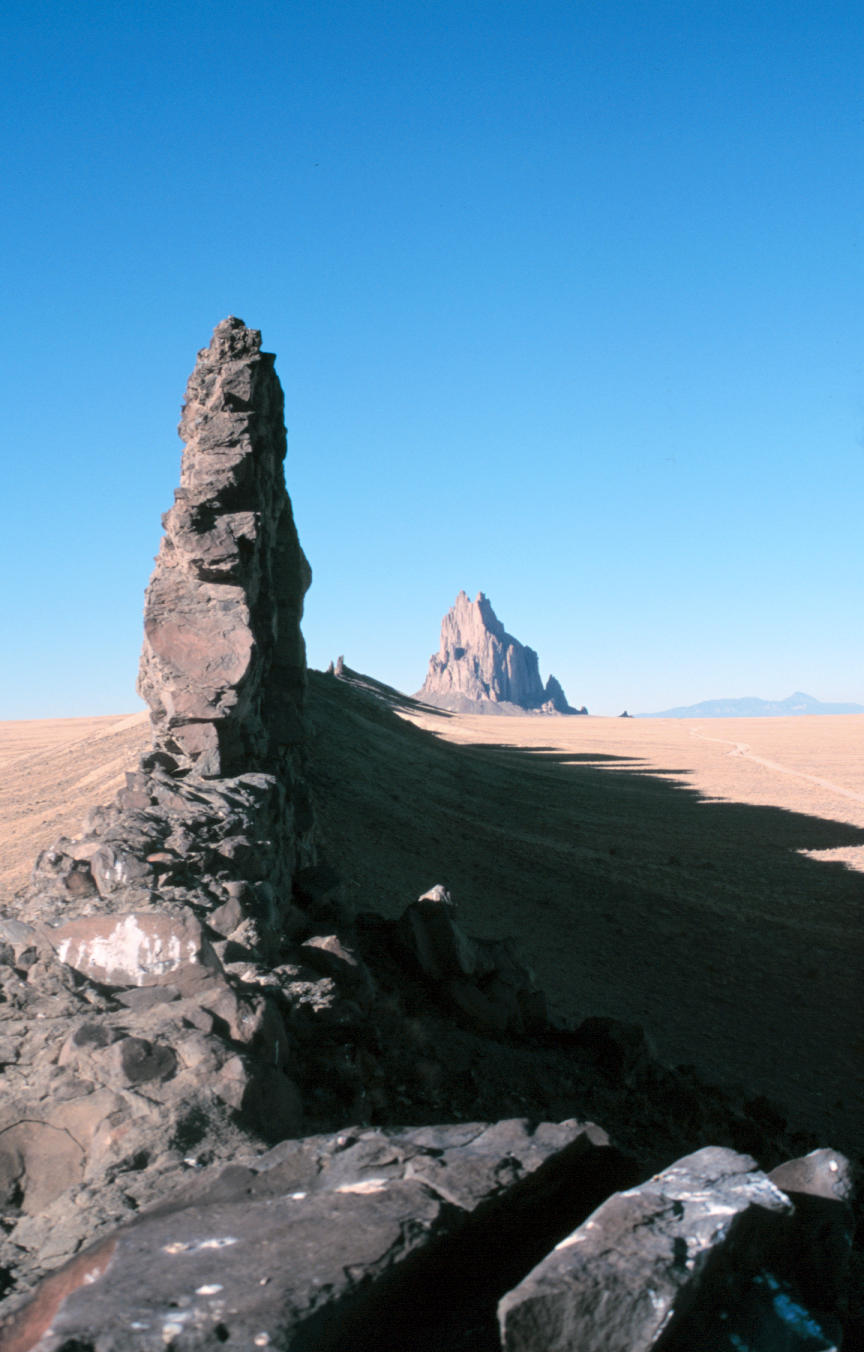
\includegraphics[width=0.3\linewidth]{images/book4/b2-shiprock-dyke.jpg}
\par\smallskip{\small 希普洛克（Shiprock）附近的一条\omterm{def:b2:magma-emplacement:bodies}{岩墙}，位于 Navajo Volcanic Field
（新墨西哥州）：\omterm{def:b2:magma-emplacement:bodies}{岩墙}岩石比其所切穿的砂岩和页岩更抗侵蚀，
如今矗立如墙；远处是火山颈，数条此类\omterm{def:b2:magma-emplacement:bodies}{岩墙}
自其向外辐射。照片：Dexter Perkins（CC0）。}
\end{omfigure}

\section{冷却与接触变质作用}

侵入体通过热传导向围岩散失热量。最简单的
模型把侵入体及其围岩视为同一导热介质，其扩散系数均匀：
扩散系数为 $\kappa$：在初始时刻，厚度为 $b$ 的岩席温度为侵入温度 $T_m$，
围岩温度为 $T_0$。热传导方程的解
（$x$ 自岩席中部量起）为
\[
T(x,t) = T_0 + \frac{T_m - T_0}{2}\left[\operatorname{erf}\frac{b/2 - x}{2\sqrt{\kappa t}}
+ \operatorname{erf}\frac{b/2 + x}{2\sqrt{\kappa t}}\right].
\]
下图给出了厚 \qty{100}{m} \omterm{def:b2:magma-emplacement:bodies}{岩床}的结果。
% ledger: delaney86b4:properties

\begin{proposition}[接触温度]\label{prop:b2:magma-emplacement:contact}
在该模型中，只要 $\sqrt{\kappa t}$ 远小于 $b$，
侵入体与围岩的接触带温度保持在
侵入温度与围岩温度的平均值 $(T_m + T_0)/2$。
\end{proposition}

\begin{proof}
在接触带（$x = b/2$）处，第一个误差函数为 $\operatorname{erf}0 = 0$，
第二个误差函数为 $\operatorname{erf}(b/(2\sqrt{\kappa t}))$，其值接近 $1$，
条件是 $b \gg 2\sqrt{\kappa t}$。于是 $T = T_0 + (T_m - T_0)/2$。
\end{proof}

温度为 \qty{1150}{\celsius} 的玄武质\omterm{def:b2:magma-emplacement:bodies}{岩墙}侵入 \qty{50}{\celsius} 的围岩，故
其接触带被加热至 \qty{600}{\celsius}。典型的结晶热
为 \qtyrange{700}{1000}{MJ/m^3}，它使\omterm{def:b2:magma-emplacement:magma}{岩浆}保持高温的时间更长，并提高这一数值：
若在 \num{1150} 至 \qty{950}{\celsius} 之间释放 \qty{900}{MJ/m^3}，同一模型给出
\qty{690}{\celsius}，而随温度变化的热导率以及含水围岩
会使这两个估计值降低 50 至 \qty{75}{\celsius}。
% ledger: delaney86b4:dike, delaney86b4:properties

\begin{omfigure}
\centering
\begin{tikzpicture}
\begin{axis}[omrecord, width=0.86\linewidth, height=6cm,
  xmin=-200, xmax=200, ymin=0, ymax=1200,
  xlabel={距岩席中部的距离（\unit{m}）},
  ylabel={温度（\unit{\celsius}）},
  legend pos=north east, legend style={font=\scriptsize},
  tick label style={font=\scriptsize}, label style={font=\small}]
\fill[gray!15] (axis cs:-50,0) rectangle (axis cs:50,1200);
\addplot[very thick, red!80!black] table[x=x_m, y=t1] {figdata/out/bachelor-2-magma-sill.dat};
\addlegendentry{1 年}
\addplot[very thick, orange!90!black] table[x=x_m, y=t2] {figdata/out/bachelor-2-magma-sill.dat};
\addlegendentry{10 年}
\addplot[very thick, blue!60!black] table[x=x_m, y=t3] {figdata/out/bachelor-2-magma-sill.dat};
\addlegendentry{50 年}
\addplot[very thick, black] table[x=x_m, y=t4] {figdata/out/bachelor-2-magma-sill.dat};
\addlegendentry{200 年}
\draw[densely dashed, gray] (axis cs:-200,625) -- (axis cs:200,625);
\node[font=\scriptsize, gray!40!black, anchor=south west] at (axis cs:-198,625) {$(T_m + T_0)/2$};
\node[font=\scriptsize, anchor=south] at (axis cs:0,20) {岩床};
\end{axis}
\end{tikzpicture}
\par\smallskip{\small 厚 \qty{100}{m} \omterm{def:b2:magma-emplacement:bodies}{岩床}（阴影部分）的传导冷却，
以 \qty{1150}{\celsius} 侵入 \qty{100}{\celsius} 的围岩，
取 $\kappa = \qty{0.7e-6}{m^2/s}$，不计潜热。接触带温度
在数十年间维持在 \qty{625}{\celsius} 附近，同时热量向围岩扩散；
两个世纪后，\omterm{def:b2:magma-emplacement:bodies}{岩床}及其周围已形成一个宽阔的温热区。}
\end{omfigure}
% ledger: delaney86b4:properties

冷却的时间尺度是热量扩散穿过侵入体所需的时间，
量级为 $(b/2)^2/\kappa$：宽 \qty{2}{m} 的\omterm{def:b2:magma-emplacement:bodies}{岩墙}约 \num{16} 天，
厚 \qty{100}{m} 的\omterm{def:b2:magma-emplacement:bodies}{岩床}约一个世纪，几千米的\omterm{def:b2:magma-emplacement:bodies}{深成岩体}约需十万年。
潜热会延长这一时间，
而要使\omterm{def:b2:magma-emplacement:magma}{岩浆}凝固而非仅仅冷却，同样会延长它。

\begin{proposition}[侵入体的凝固]\label{prop:b2:magma-emplacement:stefan}
设温度为凝固温度 $T_m$ 的\omterm{def:b2:magma-emplacement:magma}{岩浆}、单位体积潜热为 $L$，
充满 $y > 0$ 的空间，围岩温度为 $T_0$，占据 $y < 0$ 的区域，
两者的单位体积热容均为 $\rho c$，扩散系数均为 $\kappa$。
凝固前缘按 $y_s = 2\lambda\sqrt{\kappa t}$ 推进，其中 $\lambda$
是下列方程的根：
\[
\frac{L\sqrt\pi}{\rho c\,(T_m - T_0)} = \frac{e^{-\lambda^2}}{\lambda\,(1 + \operatorname{erf}\lambda)},
\]
接触带温度保持在 $T_0 + (T_m - T_0)/(1 + \operatorname{erf}\lambda)$。
厚度为 $b$ 的\omterm{def:b2:magma-emplacement:bodies}{岩床}从两壁同时凝固，
经过 $t = b^2/(16\lambda^2\kappa)$ 后完全固结。
\end{proposition}

\begin{proof}
前缘之前的\omterm{def:b2:magma-emplacement:magma}{岩浆}保持在 $T_m$，因此热量只在已凝固部分与围岩中流动，
试取 $T = T_0 + (T_m - T_0)(1 + \operatorname{erf}\xi)/(1 +
\operatorname{erf}\lambda)$，其中 $\xi = y/(2\sqrt{\kappa t})$。凡关于 $\xi$ 的函数，
若形如 $\alpha + \beta\operatorname{erf}\xi$，则都满足热传导方程；
该解在围岩深处趋于 $T_0$（$\xi \to -\infty$），前缘处等于 $T_m$（$\xi = \lambda$）。
在 $y = 0$ 处，它给出所述的接触带温度。在前缘上，
凝固前进时释放的潜热 $L\,dy_s/dt = L\lambda\sqrt{\kappa/t}$，
单位面积、单位时间的潜热必须由传导带走，即 $k\,\partial T/\partial y = k(T_m -
T_0)\,e^{-\lambda^2}/[(1 + \operatorname{erf}\lambda)\sqrt{\pi\kappa t}]$。令两者相等，
并利用 $k = \rho c\kappa$，即得 $\lambda$ 所满足的方程。\omterm{def:b2:magma-emplacement:bodies}{岩床}的每一壁
各自生长一个前缘，只要中心保持在 $T_m$，彼此互不影响；两个
前缘在 $2\lambda\sqrt{\kappa t} = b/2$ 时相遇。
\end{proof}

取玄武岩的潜热、围岩温度约为 \qty{100}{\celsius}，
$\lambda$ 约为 $0.65$：厚 \qty{100}{m} 的\omterm{def:b2:magma-emplacement:bodies}{岩床}约需
七十年凝固，其接触带温度在此期间维持在 \qty{740}{\celsius} 附近，
而非 \qty{625}{\celsius}。周末问题将详细计算这一情形。
由于时间随厚度的平方增长，厚度为十倍的\omterm{def:b2:magma-emplacement:bodies}{岩床}
所需时间是原来的一百倍。

\begin{definition}[接触变质晕及其岩石]\label{def:b2:magma-emplacement:aureole}
\emph{冷凝边}\index{冷凝边}是侵入体细粒或玻璃质的
边缘，\omterm{def:b2:magma-emplacement:magma}{岩浆}在此与较冷的围岩相接触而快速冷却。
\emph{接触变质晕}\index{接触变质晕}是侵入体周围的围岩带，
该围岩带受侵入体热量作用而发生变质。\emph{角岩}\index{角岩}是
泥岩和火山岩在接触变质晕中转变而成的坚硬、细粒、无片理的岩石。
\emph{矽卡岩}\index{矽卡岩}是高温\omterm{def:b2:magma-emplacement:magma}{岩浆}流体
与碳酸盐围岩发生反应所形成的岩石，沉淀出钙–铁–镁
硅酸盐（如石榴子石和辉石），常伴有磁铁矿和金属硫化物。
\end{definition}
% ledger: earle:intrusive-bodies, earle:skarn

\omterm{def:b2:magma-emplacement:aureole}{接触变质晕}的宽度从小\omterm{def:b2:magma-emplacement:bodies}{岩墙}和\omterm{def:b2:magma-emplacement:bodies}{岩床}周围的几厘米，
到大型岩株周围的数十米不等，接触变质作用的温度范围约为
\qty{300}{\celsius} 至 \qty{800}{\celsius} 以上。泥岩变为\omterm{def:b2:magma-emplacement:aureole}{角岩}，
石灰岩变为大理岩，砂岩变为石英岩。侵入到本已炽热岩石深处的\omterm{def:b2:magma-emplacement:magma}{岩浆}
几乎不形成变质晕：变质晕的宽度取决于侵入体的大小和温度，
以及围岩的温度，这一点与冷却模型的预测一致（见\cref{exo:b2:magma-emplacement:12}）。
变质晕中生长的矿物，
及其所指示的温度，属于\cref{ch:b2:metamorphic-facies}的内容；
\omterm{def:b2:magma-emplacement:aureole}{矽卡岩}富集的金属则属于\cref{ch:b2:ore-deposits}。
% ledger: earle:skarn

\begin{inthefield}[读取岩墙的接触带]
\begin{minipage}[t]{0.6\linewidth}\vspace{0pt}
\omterm{def:b2:magma-emplacement:bodies}{岩墙}出露时，地质学家首先沿其与围岩的接触带追踪。
若某一边缘比\omterm{def:b2:magma-emplacement:bodies}{岩墙}中心更细粒或更玻璃质，
则表明\omterm{def:b2:magma-emplacement:magma}{岩浆}是贴着冷岩石快速冷却的；一条在不列颠哥伦比亚省海岸研究的\omterm{def:b2:magma-emplacement:bodies}{岩墙}
宽 \qty{25}{cm}，其\omterm{def:b2:magma-emplacement:aureole}{冷凝边}厚 \qty{2}{cm}。接下来检查紧邻接触带的围岩是否发生烘烤：
颜色改变、岩石变硬，以及远离\omterm{def:b2:magma-emplacement:bodies}{岩墙}渐渐消失的新矿物。
烘烤带和\omterm{def:b2:magma-emplacement:aureole}{冷凝边}的宽度与\omterm{def:b2:magma-emplacement:bodies}{岩墙}宽度相比，可以指示\omterm{def:b2:magma-emplacement:bodies}{岩墙}侵入时
围岩有多热；没有\omterm{def:b2:magma-emplacement:aureole}{冷凝边}也没有变质晕的\omterm{def:b2:magma-emplacement:bodies}{岩墙}，
是侵入到本已炽热岩石中的。
沿\omterm{def:b2:magma-emplacement:bodies}{岩墙}自边缘至中心横向采样，
用于分析熔体的地球化学成分，
以及晶体的大小。
\end{minipage}\hfill
\begin{minipage}[t]{0.36\linewidth}\vspace{0pt}
\centering
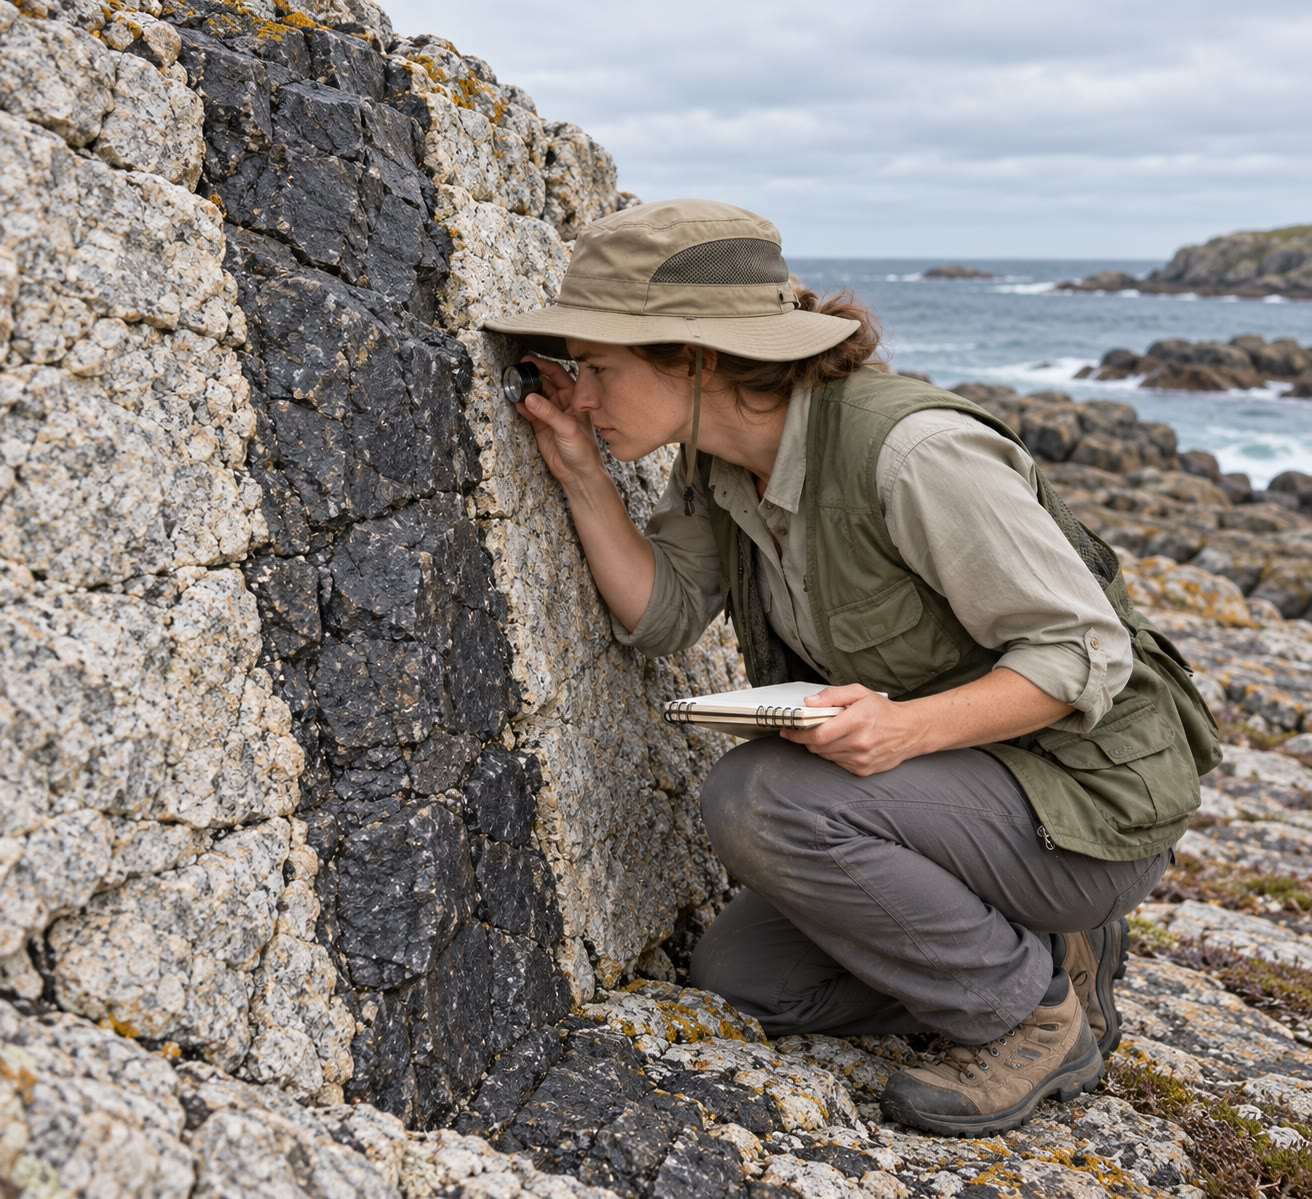
\includegraphics[width=\linewidth]{images/book4/ai/b2-dyke-contact.jpg}
\par\smallskip{\scriptsize 地质学家正在考察深色\omterm{def:b2:magma-emplacement:bodies}{岩墙}与浅色围岩的接触带
（AI 生成插图）。}
\end{minipage}
\end{inthefield}
% ledger: earle:intrusive-bodies

\section{练习}

\begin{exercise}[$\star$]\label{exo:b2:magma-emplacement:1}
对于含水花岗质熔体，拟合测量数据得到的方程为
$\log_{10}\eta = [-3.545 + 0.833\ln w] + [9601 - 2368\ln w]/\{T - [195.7 + 32.25\ln
w]\}$，其中 $\eta$ 的单位为 \unit{Pa.s}，$w$ 为水的质量百分含量，$T$
为开尔文温度。计算温度为 \qty{800}{\celsius} 时的 $\log_{10}\eta$，
分别取 $w = 1$ 与 $w = 4$，并求多出的三个百分点的水使黏度降低的倍数。
\end{exercise}
% ledger: hd96:model

\begin{exercise}[$\star$]\label{exo:b2:magma-emplacement:2}
利用平方根定律，流纹岩取 $s = 0.44$，玄武岩取 $s = 0.34$，
单位为质量百分数每 $\sqrt{\unit{MPa}}$，求含水 \qty{6}{\percent} 的流纹岩和
含水 \qty{0.5}{\percent} 的玄武岩的饱和压强，
以及它们在密度为 \qty{2600}{kg/m^3} 的地壳中对应的深度，
其中 $g = \qty{9.81}{m/s^2}$。
\end{exercise}

\begin{exercise}[$\star$]\label{exo:b2:magma-emplacement:3}
计算温度为 \qty{1150}{\celsius} 的玄武岩\omterm{def:b2:magma-emplacement:bodies}{岩墙}侵入
\qty{50}{\celsius} 围岩时的接触带温度，再计算侵入 \qty{400}{\celsius} 围岩时的接触带温度。
两条\omterm{def:b2:magma-emplacement:bodies}{岩墙}中哪一条的\omterm{def:b2:magma-emplacement:aureole}{冷凝边}更宽？
\end{exercise}

\begin{exercise}[$\star$]\label{exo:b2:magma-emplacement:4}
说出每个岩体的名称。（a）厚 \qty{30}{m} 的粗玄岩岩席，位于两层
延伸超过 \qty{20}{km} 的砂岩层之间。（b）一垂直的玄武岩\omterm{def:b2:magma-emplacement:bodies}{岩墙}，宽 \qty{2}{m}，
切穿水平石灰岩层。（c）出露面积达 \qty{2000}{km^2} 的花岗岩体，
由十几个不同时代的单元构成。（d）一斑岩透镜体，直径 \qty{1}{km}，
底部平坦，其上岩层向上拱起。（e）一层水平的
玄武岩岩席，位于花岗岩中。
\end{exercise}

\begin{exercise}[$\star\star$]\label{exo:b2:magma-emplacement:5}
某玄武质熔体满足 $\eta_{\ell} = \qty{100}{Pa.s}$。利用爱因斯坦–罗斯科
关系式（$R = 1.35$），计算下列晶体含量下\omterm{def:b2:magma-emplacement:magma}{岩浆}的黏度：
\qty{5}{\percent}、\qty{20}{\percent}、\qty{40}{\percent} 和 \qty{60}{\percent} 的
晶体，并将第一个结果与爱因斯坦稀悬浮体公式比较。关系式预测在
何种晶体含量下\omterm{def:b2:magma-emplacement:magma}{岩浆}发生堵塞？
\end{exercise}

\begin{exercise}[$\star\star$]\label{exo:b2:magma-emplacement:6}
密度比围岩小 \qty{300}{kg/m^3} 的\omterm{def:b2:magma-emplacement:magma}{岩浆}沿\omterm{def:b2:magma-emplacement:bodies}{岩墙}上升。
（a）对玄武岩（$\eta = \qty{100}{Pa.s}$，$\rho = \qty{2700}{kg/m^3}$），在
宽 \qty{1}{m} 的\omterm{def:b2:magma-emplacement:bodies}{岩墙}中，计算平均速度、每米\omterm{def:b2:magma-emplacement:bodies}{岩墙}的通量、
雷诺数，以及上升 \qty{10}{km} 所需的时间。（b）对黏度为 \qty{e6}{Pa.s} 的流纹质\omterm{def:b2:magma-emplacement:magma}{岩浆}，
分别计算在宽 \qty{1}{m} 与宽 \qty{10}{m} \omterm{def:b2:magma-emplacement:bodies}{岩墙}中的上升时间。（c）一条
宽 \qty{1}{m} 的\omterm{def:b2:magma-emplacement:bodies}{岩墙}，其热量散失的时间量级为 $(w/2)^2/\kappa$，其中 $\kappa =
\qty{1e-6}{m^2/s}$。三种上升过程中哪一种可能成功？
\end{exercise}

\begin{exercise}[$\star\star$]\label{exo:b2:magma-emplacement:7}
一密度为 \qty{2400}{kg/m^3}、温度为 \qty{900}{\celsius} 的\omterm{def:b2:magma-emplacement:magma}{岩浆}，
释放出其质量的 \qty{1}{\percent} 作为水蒸气。将水蒸气视为理想气体，
（$R = \qty{8.314}{J/(mol.K)}$，\qty{18.015}{g/mol}），计算\omterm{def:b2:magma-emplacement:magma}{岩浆}中
气体的体积分数，压强分别为 \qty{100}{MPa}、\qty{10}{MPa} 和 \qty{0.1}{MPa}。三个结果中
哪一个最不可靠？为什么？
\end{exercise}

\begin{exercise}[$\star\star$]\label{exo:b2:magma-emplacement:8}
在某盆地中，岩石密度随深度 $z$ 增大，满足 $\rho(z) =
2300 + 60\,z$（\unit{kg/m^3}，$z$ 的单位为 \unit{km}），直至 \qty{10}{km} 深度。（a）求
密度为 \qty{2650}{kg/m^3} 的玄武质熔体的\omterm{def:b2:magma-emplacement:ascent}{中性浮力面}所在深度。（b）本章
的密度模型表明，溶解水每增加 \qty{1}{\percent}，玄武质熔体
密度约降低 \qty{70}{kg/m^3}。若熔体再多含 \qty{1}{\percent} 的水，
它将在何处停止上升？（c）位于\omterm{def:b2:magma-emplacement:ascent}{中性浮力面}以下
\qty{2}{km} 处的干熔体，每立方米所受浮力为多大？
\end{exercise}

\begin{exercise}[$\star\star$]\label{exo:b2:magma-emplacement:9}
设一花岗质\omterm{def:b2:magma-emplacement:ascent}{底辟}体，半径为 \qty{1}{km}，密度差为
\qty{300}{kg/m^3}，穿过黏度为 \qty{e19}{Pa.s} 的下地壳上升。计算
其斯托克斯速度（刚性球体），以毫米每年为单位，以及上升
\qty{10}{km} 所需的时间。与其冷却时间尺度 $a^2/\kappa$ 比较，其中 $\kappa
= \qty{1e-6}{m^2/s}$。你能得出什么结论？
\end{exercise}

\begin{exercise}[$\star\star\star$]\label{exo:b2:magma-emplacement:10}
水在熔体中既以分子形式溶解，$x_m = K_1 f$，又以羟基形式溶解，
$x_{\mathrm{OH}}^2 = K_2 x_m$（熔体中的氧大量过量），故
溶解水总量为 $x = x_m + x_{\mathrm{OH}}/2$。（a）将 $x$ 写成
$f$ 的函数，并证明它按 $\sqrt f$ 变化（低 $f$ 时），
按 $f$ 变化（高 $f$ 时）。（b）两种形式的水含量相等时，对应的逸度为多少？（c）
取 $K_1 = \qty{1e-4}{MPa^{-1}}$，$K_2 = 0.2$，计算该逸度，以及
\qty{100}{MPa} 时以羟基形式溶解的水所占份额。
\end{exercise}

\begin{exercise}[$\star\star\star$]\label{exo:b2:magma-emplacement:11}
一花岗质\omterm{def:b2:magma-emplacement:bodies}{深成岩体}体积为 \qty{1000}{km^3}，历时 \qty{4}{Ma} 逐步形成。（a）计算
其平均\omterm{def:b2:magma-emplacement:magma}{岩浆}供给速率，以 \unit{km^3} 每年和 \unit{m^3} 每秒表示。（b）一条
单条\omterm{def:b2:magma-emplacement:bodies}{岩墙}长 \qty{1}{km}、宽 \qty{2}{m}，平均速度为
\qty{0.8}{m/s}，为其供给\omterm{def:b2:magma-emplacement:magma}{岩浆}。该\omterm{def:b2:magma-emplacement:bodies}{岩墙}需要多长时间才能输送完整个\omterm{def:b2:magma-emplacement:bodies}{岩基}？
这段时间占 \qty{4}{Ma} 的比例是多少？（c）若该\omterm{def:b2:magma-emplacement:bodies}{岩基}由
厚 \qty{20}{m}、长宽各为 \qty{10}{km} 的岩席构成，需要多少层岩席，
以及相邻两层岩席平均相隔多长时间？（d）取
$\lambda = 0.65$，$\kappa = \qty{0.7e-6}{m^2/s}$，求一层岩席
固结所需的时间。该\omterm{def:b2:magma-emplacement:bodies}{岩基}是否曾经是一个单一的大体量\omterm{def:b2:magma-emplacement:magma}{岩浆}体？
\end{exercise}

\begin{exercise}[$\star\star\star$]\label{exo:b2:magma-emplacement:12}
在远离宽度为 $b$ 的细\omterm{def:b2:magma-emplacement:bodies}{岩墙}处（距离 $x \gg b$），其热效应相当于一个
瞬时平面源：$T - T_0 = (T_m - T_0)\,b\,e^{-x^2/(4\kappa
t)}/\sqrt{4\pi\kappa t}$。（a）证明：距离 $x$ 处的温度在
$t^* = x^2/(2\kappa)$ 时最高，且该最大升温为 $\Delta T_{\max} = (T_m -
T_0)\,b/(x\sqrt{2\pi e})$。（b）对宽 \qty{2}{m} 的\omterm{def:b2:magma-emplacement:bodies}{岩墙}，取 $T_m - T_0 =
\qty{1100}{K}$，岩石升温至多 \qty{100}{K} 的距离为多少，
以及发生在何时（$\kappa = \qty{0.7e-6}{m^2/s}$）？（c）细\omterm{def:b2:magma-emplacement:bodies}{岩墙}的
\omterm{def:b2:magma-emplacement:aureole}{接触变质晕}为何如此窄？
\end{exercise}

\section{问题：高原下的岩席}

\begin{problem}[{周末问题——追踪玄武质岩浆从供给岩墙到岩席的过程，
其中的水以及岩席固结所需的时间}]
\label{pb:b2:magma-emplacement:1}
在一虚构高原之下，平均密度为
\qty{2450}{kg/m^3} 的沉积物（页岩与砂岩）位于 \qty{3.0}{km} 深处，覆于
密度为 \qty{2800}{kg/m^3} 的结晶基底之上。一玄武质\omterm{def:b2:magma-emplacement:magma}{岩浆}从 \qty{15}{km} 深处经
宽 \qty{2.0}{m} 的\omterm{def:b2:magma-emplacement:bodies}{岩墙}上升，并沿沉积层底部铺展，形成粗玄岩岩席，
厚 \qty{100}{m}。已知数据：侵入温度 \qty{1150}{\celsius}；熔体
黏度定律 $\log_{10}\eta = -4.55 + 5510/(T - 611)$（$T$ 以开尔文为单位）；熔体
含水时的密度为 \qty{2710}{kg/m^3}；晶体体积分数为 \qty{20}{\percent}
（爱因斯坦–罗斯科关系，$R = 1.35$）；溶解水 \qty{0.40}{\percent}，溶解度
$s = 0.34$，单位为质量百分数每 $\sqrt{\unit{MPa}}$；岩席处围岩温度
\qty{100}{\celsius}；$\kappa = \qty{0.7e-6}{m^2/s}$，$\rho c = \qty{2.5}{MJ/(m^3.K)}$，
潜热 \qty{900}{MJ/m^3}，并视\omterm{def:b2:magma-emplacement:magma}{岩浆}在其
侵入温度下固结；$g = \qty{9.81}{m/s^2}$；一年取 \qty{3.156e7}{s}。

\medskip\noindent\textbf{第一部分——\omterm{def:b2:magma-emplacement:magma}{岩浆}。}
\begin{enumerate}
\item 计算 \qty{1150}{\celsius} 时熔体的 $\log_{10}\eta$ 与 $\eta$
（\qty{1423}{K}）。
\item 求 \qty{1100}{\celsius} 时的同一结果。在这 \qty{50}{K} 的温降中，
黏度改变了多少倍？
\item 计算含晶体的\omterm{def:b2:magma-emplacement:magma}{岩浆}在
\qty{1150}{\celsius} 时的黏度。
\item 爱因斯坦–罗斯科关系在晶体含量为多少时
会使\omterm{def:b2:magma-emplacement:magma}{岩浆}发生堵塞？请与野外估计的整体流动终止值进行比较。
\item 计算\omterm{def:b2:magma-emplacement:magma}{岩浆}与基底之间的密度差，以及
\omterm{def:b2:magma-emplacement:magma}{岩浆}与沉积物之间的密度差。
\item 计算岩席所在深度处的静岩压力。
\end{enumerate}

\noindent\textbf{第二部分——沿\omterm{def:b2:magma-emplacement:bodies}{岩墙}上升。}
\begin{enumerate}[resume]
\item 计算驱动\omterm{def:b2:magma-emplacement:magma}{岩浆}
穿过基底的浮力压强梯度 $\Delta\rho\,g$。
\item 计算\omterm{def:b2:magma-emplacement:magma}{岩浆}在\omterm{def:b2:magma-emplacement:bodies}{岩墙}中的平均速度。
\item 计算每米\omterm{def:b2:magma-emplacement:bodies}{岩墙}的通量，以及\omterm{def:b2:magma-emplacement:bodies}{岩墙}长
\qty{1.0}{km}时的总通量。
\item 计算该流动的雷诺数，并判断它是否为层流。
\item \omterm{def:b2:magma-emplacement:magma}{岩浆}从 \qty{15}{km} 上升到 \qty{3.0}{km} 需要多长时间？
\item 与\omterm{def:b2:magma-emplacement:bodies}{岩墙}散失其热量所需的时间尺度 $(w/2)^2/\kappa$ 相比较，
\omterm{def:b2:magma-emplacement:bodies}{岩墙}能否保持张开？
\item 试解释\omterm{def:b2:magma-emplacement:magma}{岩浆}为何在 \qty{3.0}{km} 处停止上升并向两侧铺展，
并用本章的术语作答。
\end{enumerate}

\noindent\textbf{第三部分——水。}
\begin{enumerate}[resume]
\item 计算熔体中水的饱和压强，以及
达到该压强处在沉积物中的深度。
\item 在\omterm{def:b2:magma-emplacement:bodies}{岩床}所在深度，熔体最多能容纳多少水？\omterm{def:b2:magma-emplacement:bodies}{岩床}
\omterm{def:b2:magma-emplacement:magma}{岩浆}是否会出溶水？
\item \omterm{def:b2:magma-emplacement:bodies}{岩床}\omterm{def:b2:magma-emplacement:aureole}{冷凝边}中的气泡主要含 CO$_2$。试解释。
\item 若全部 \qty{0.40}{\percent} 的水在
\qty{1150}{\celsius} 与 \qty{0.1}{MPa} 条件下于地表释出，
则蒸气将占\omterm{def:b2:magma-emplacement:magma}{岩浆}的多大体积分数（视为理想气体）？
\end{enumerate}

\noindent\textbf{第四部分——冷却与凝固。}
\begin{enumerate}[resume]
\item 忽略潜热，计算\omterm{def:b2:magma-emplacement:bodies}{岩床}的接触温度。
\item 忽略潜热，计算顶部接触面之上 \qty{10}{m} 处
在侵入后 \num{10}~年时的温度。
\item 同一模型：计算\omterm{def:b2:magma-emplacement:bodies}{岩床}中部在
侵入后 \num{10}~年和 \num{50}~年时的温度。
\item 同一模型：计算顶部接触面以上 \qty{80}{m} 处
在 \num{300}、\num{363} 和 \num{420} 年后的温度。
该处岩石是否曾达到 \qty{300}{\celsius}？
\item 计算\omterm{def:b2:magma-emplacement:bodies}{岩床}的 $L\sqrt\pi/(\rho c\,(T_m - T_0))$。
\item 计算 $e^{-\lambda^2}/(\lambda(1 + \operatorname{erf}\lambda))$ 在 $\lambda = 0.64$、
$0.65$ 和 $0.66$ 处的值（$\operatorname{erf}0.64 = 0.6346$，$\operatorname{erf}0.65 = 0.6420$，
$\operatorname{erf}0.66 = 0.6494$），并将 $\lambda$ 保留到两位小数。
\item 计入潜热，计算\omterm{def:b2:magma-emplacement:bodies}{岩床}凝固过程中的
接触温度。为何它比第 18 题中的结果更高？
\item 以年为单位，计算时间尺度 $(b/2)^2/\kappa$。
\item 计算\omterm{def:b2:magma-emplacement:bodies}{岩床}凝固所需的时间（以年为单位），此即本题的关键数值，
并解释为何它比上一题中的时间尺度更短，
尽管仍须移走潜热。
\end{enumerate}
\end{problem}
% ledger: grd08:model, kolz22:einstein-roscoe, glazner04:tuolumne, moore98:h2o, lowenstern01:co2, delaney86b4:properties
